\documentclass{article}
\usepackage[utf8]{inputenc}
\usepackage{relsize}
\usepackage{geometry}
\usepackage{tikz}
\usetikzlibrary{automata, positioning, arrows}
\tikzset{node distance=2.5cm, % Minimum distance between two nodes. Change if necessary.
every state/.style={ % Sets the properties for each state
semithick,
fill=gray!10},
initial text={}, % No label on start arrow
double distance=2pt, % Adjust appearance of accept states
every edge/.style={ % Sets the properties for each transition
draw,->,>=stealth', % Makes edges directed with bold arrowheads
auto,semithick}}



\geometry{
 a4paper,
 total={170mm,257mm},
 left=20mm,
 top=20mm,
}

\title{Homework 1\\[0.2em]\smaller{}CSC 445-01: Theory of Computation}
\author{Matthew Mabrey, Luke Kurlandski}
\date{\today}

\begin{document}

\maketitle

\section*{Question I}

We will show that $A=B$ using three proofs by contradiction. First, it is helpful to expand the following
$$
A \times B = \biggr \{ (a,b) | a \in A, b \in B \biggr \}
$$
$$
B \times A = \biggr \{ (b,a) | b \in B, a \in A \biggr \}
$$
Thus the original condition is
$$
A \times B \subseteq B \times A
$$
$$
\biggr \{ (a,b) | a \in A, b \in B \biggr \} \subseteq \biggr \{ (b,a) | b \in B, a \in A \biggr \}
$$

\subsection*{1}
Suppose $A \not \subseteq B$. Then $\exists \; a \in A $ where $ (a \not \in B) $. Then $\exists \; (a, b) \in A \times  B $ where $ ((a, b) \not \in B \times  A ) $. This defies the original condition. We have proven
$$A \subseteq B$$

\subsection*{2}
Suppose $B \not \subseteq A$. Then $\exists \; b \in B $ where $ (b \not \in A) $. Then $\exists \; (a, b) \in A \times  B $ where $ ((a, b) \not \in B \times  A ) $. This defies the original condition. We have proven
$$B \subseteq A$$

\subsection*{3}
Suppose $A \neq B$. Then one of the following two statements must be true:
\begin{enumerate} 
\item $\exists \; a \in A $ where $ (a \not \in B) $, which violates $A \subseteq B$
\item $\exists \; b \in B $ where $ (b \not \in A) $, which violates $B \subseteq A$
\end{enumerate}
Thus we have proven
$$A = B$$

\section*{Question II}

Given a relation on the set of all nonempty subsets of \textit{N} tell whether it is reflexive, symmetric, or transitive.

\subsection*{a} 
\textit{R} is defined by: \textit{ARB} if and only if \textit{A} $\subseteq$ \textit{B} 
\\\\  - Reflexive because the relation over any given element subset relates every element to itself. In our case \textit{X} $\subseteq$ \textit{X} holds true since a set will always be a subset of itself.
\\\\  - Not symmetric because an element \textit{X} being a subset of the element Y only guarantees that \textit{Y} contains all of \textit{X}'s elements but not vice versa. So every \textit{XRY} $\neq$ \textit{YRX}. 
\\\\  - Transitive because an element \textit{X} can only be a subset of \textit{Y} if it contains all of \textit{X}'s elements. Then for \textit{Y} to be a subset of \textit{Z} it must contain all of \textit{Y}'s elements. Thus guaranteeing that all of \textit{X}'s elements are contained within \textit{Z} therefore making \textit{X} $\subseteq$ \textit{Z} and the relation \textit{XRY} $\land$ \textit{YRZ} $\rightarrow$ \textit{XRZ} hold true.  
    
\subsection*{b}
\textit{R} is defined by: \textit{ARB} if and only if \textit{A} $\cap$ \textit{B} $\neq \theta$  
\\\\  - Reflexive because \textit{X} $\cap$ \textit{X} will never be an empty set since the parent set only contains nonempty subsets of \textit{N} and so \textit{X} intersecting with itself will always contain at least one element.
\\\\  - Symmetric because the relation in this case does not care about order since if the intersection of two sets \textit{X} $\cap$ \textit{Y} results in a nonempty set then \textit{Y} $\cap$ \textit{X} will also yield the same result set.
\\\\  - Not transitive because while \textit{X} $\cap$ \textit{Y} may result in a nonempty set based on some subset of shared elements, the intersection \textit{Y} $\cap$ \textit{Z} could result in a nonempty set based on a different subset of shared elements. Therefore the transitive relation \textit{XRY} $\land$ \textit{YRZ} $\rightarrow$ \textit{XRZ} would not always hold true.
    
\subsection*{c}
\textit{R} is defined by: \textit{ARB} if and only if 1 $\in$ \textit{A} $\cap$ \textit{B} 
\\\\  - Not Reflexive because if $1 \not \in x$, then $1 \not \in x \cap x$
\\\\  - Symmetric because the order of the sets in the intersection \textit{X} $\cap$ \textit{Y} doesn't matter and if the result set contains 1 then the intersection \textit{Y} $\cap$ \textit{X} set will also contain 1.
\\\\  - Transitive because if the result set of \textit{X} $\cap$ \textit{Y} contains 1 and the result set of \textit{Y} $\cap$ \textit{Z} also contains 1 then all 3 sets must contain 1 and so \textit{X} $\cap$ \textit{Z} will also contain one and the transitive relation holds true.

\section*{Question III}
We will prove
$$
P(n) \colon \sum^n_{i=1} \frac{1}{i(i+1)} = \frac{n}{n+1} \;\; \biggr | \;\; n \geq 0, n \in Z
$$
Base case:
\begin{eqnarray*}
P(0) &\colon& \sum^n_{i=1} \frac{1}{i(i+1)} = \frac{n}{n+1} \\
&\colon& \sum^0_{i=1} \frac{1}{i(i+1)} = \frac{0}{0+1} \\
&\colon& 0 = 0 \\
&\colon& \textrm{TRUE}
\end{eqnarray*}
Inductive Hypothesis:
$$
P(k) \colon \sum^k_{i=1} \frac{1}{i(i+1)} = \frac{k}{k+1} \;\; \biggr | \;\; k \geq 0, k \in Z
$$
Induction:
\begin{eqnarray*}
P(k+1) &\colon& \;\; \frac{(k+1)}{(k+1)+1} = \sum^{k+1}_{i=1} \frac{1}{i(i+1)}  \\
&\colon& \;\; \frac{k+1}{k+2} = \sum^k_{i=1} \frac{1}{i(i+1)} + \frac{1}{(k+1)((k+1)+1)} \\
&\colon& \;\; \frac{k+1}{k+2} = \frac{k}{k+1} + \frac{1}{(k+1)(k+2)} \\ 
&\colon& \;\; \frac{k+1}{k+2} = \frac{k(k+2) + 1}{(k+1)(k+2)} \\ 
&\colon& \;\; \frac{k+1}{k+2} = \frac{(k+1)^2}{(k+1)(k+2)} \\
&\colon& \;\; \frac{k+1}{k+2} = \frac{k+1}{(k+2)} \\
P(k+1) &\colon& \textrm{TRUE}
\end{eqnarray*}
Conclusion:
$$
\left (  P(0) \; \land \; \biggr ( P(k) \rightarrow P(k+1) \biggr ) \right ) \rightarrow P(n) 
$$

\section*{Question IV}

\subsection*{Truth Table}
\begin{displaymath}
\begin{array}{c c|c|c|c|c|c} % bars control columns
p & q & 
(p \rightarrow q) \land (p \rightarrow \neg q) & 
p \land (p \rightarrow q) & 
(p \rightarrow q) \land (\neg p \rightarrow q) &
p \iff (p \iff q) &
q \land (p \rightarrow q)
\\ 
\hline
T & T & F & T & T & T & T \\
T & F & F & F & F & F & F \\
F & T & T & F & T & T & T \\
F & F & T & F & F & F & F 
\end{array}
\end{displaymath}

\subsection*{Equivalence}
\begin{displaymath}
\begin{array}{c|c|c} % bars control columns
Problem & Original & Simplified \\
\hline
a & (p \rightarrow q) \land (p \rightarrow \neg q) & \neg p \\ 
b & p \land (p \rightarrow q) & p \land q \\
c & (p \rightarrow q) \land (\neg p \rightarrow q) & q \\
d & p \iff (p \iff q) & q \\
e & q \land (p \rightarrow q) & q
\end{array}
\end{displaymath}

\section*{Question V}

\[ \textrm{Given } P = \theta, Q=\{\epsilon\}, R=\{aba, bcb, cac\}, \textrm{ and } S=\{aba, abc, abb\}\]

\subsection{1}
\textit{P $\subset$ Q} is correct because $\theta$ is a proper subset all of sets (besides itself) since all elements contained in P are contained within Q, while P $\neq$ Q.

\subsection{2}
\textit{R $\cap$ S} = \{\textit{aba}\} because $\cap$ is the intersection of both sets and the only element both sets share is \textit{aba}.

\subsection{3}
\textit{R $\triangle$ S} = \{\textit{bcb, cac, abc, abb}\} because $\triangle$ is the disjoint union of both sets. In other words, the set of elements from both sets that are not shared between them. Thus the resulting set is every element besides the shared element \textit{aba} from the previous problem.

\subsection{4}
\textit{$\vert\vert$R $\vert\vert$} = 3 because the cardinality of a set is the number of elements contained within within the set.

\section*{Question VI}

\[ \textrm{Given } P = (x \rightarrow y) \land (y \rightarrow z) \textrm{ where x, y, and z are boolean variables}\]

\subsection{1} 
The value of \textit{P} is false when \textit{x, z = true} and \textit{y = false} because the first implication \textit{(x $\rightarrow$ y)} in the \textit{AND} statement evaluates to false. This is because the hypothesis in the implication is true while the conclusion is false, which is the only case where the implication will evaluate to false.

\subsection{2} 
The value of \textit{P} is again false when \textit{y = true} and \textit{x, z = false} because the second implication \textit{(y $\rightarrow$ z)} in the \textit{AND} statement evaluates to false. The same reasoning as above applies where the hypothesis in the implication is true, while the conclusion is false, causing the implication to be false.

\section*{Question VII}

\subsection{1} 

Let the 4-state finite automaton that accepts the words over \{\textit{a}, \textit{b}\} that end with \textit{aba} be formally defined by

\[
M = \left(\{q_0, q_1, q_2, q_3\}, \{\textit{a},
\textit{b}\}, \delta, q_0, \{q_3\} \right),
\]
\[\textrm{where } \delta \textrm{ is given by} \] 
\begin{center}
    \begin{tabular}{c|cc}
    & \textit{a} & \textit{b}\\ \hline
    $q_0$ & $q_1$ & $q_0$ \\
    $q_1$ & $q_1$ & $q_2$ \\
    $q_2$ & $q_3$ & $q_0$ \\
    $q_3$ & $q_1$ & $q_2$
    \end{tabular}
\end{center}

The state diagram then constructed from this definition is thus

\begin{center}
    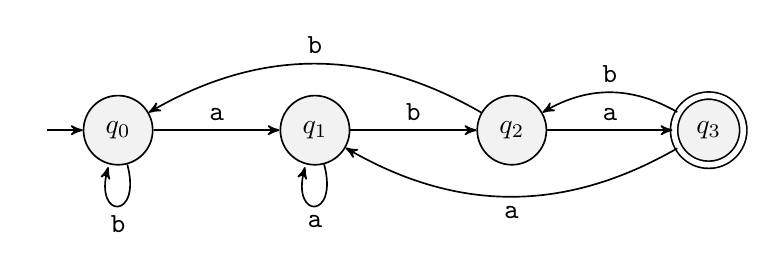
\begin{tikzpicture}
    \node[state, initial] (q0) {$q_0$};
    \node[state, right of=q0] (q1) {$q_1$};
    \node[state, right of=q1] (q2) {$q_2$};
    \node[state, accepting, right of=q2] (q3) {$q_3$};
    \draw (q0) edge node {\tt a} (q1);
    \draw (q0) edge[loop below] node {\tt b} (q0);
    \draw (q1) edge[loop below] node {\tt a} (q1);
    \draw (q1) edge node {\tt b} (q2);
    \draw (q2) edge node {\tt a} (q3);
    \draw (q2) edge[above, bend right] node {\tt b} (q0);
    \draw (q3) edge[below, bend left] node {\tt a} (q1);
    \draw (q3) edge[above, bend right] node {\tt b} (q2);
    \end{tikzpicture}
\end{center}

\subsection{2}

Let the 6-state finite automaton that accepts the words over \{0, 1\} that contain either 000 or 111 be formally defined by

\[
M = \left(\{q_0, q_1, q_2, q_3, q_4, q_5\}, \{0,
1\}, \delta, q_0, \{q_5\} \right),
\]
\[\textrm{where } \delta \textrm{ is given by} \] 
\begin{center}
    \begin{tabular}{c|cc}
    & \textrm{0} & \textrm{1}\\ \hline
    $q_0$ & $q_1$ & $q_0$ \\
    $q_1$ & $q_1$ & $q_2$ \\
    $q_2$ & $q_3$ & $q_0$ \\
    $q_3$ & $q_1$ & $q_2$ \\
    $q_4$ & $q_1$ & $q_2$ \\
    $q_5$ & $q_1$ & $q_2$
    \end{tabular}
\end{center}

The state diagram then constructed from this definition is thus

\begin{center}
    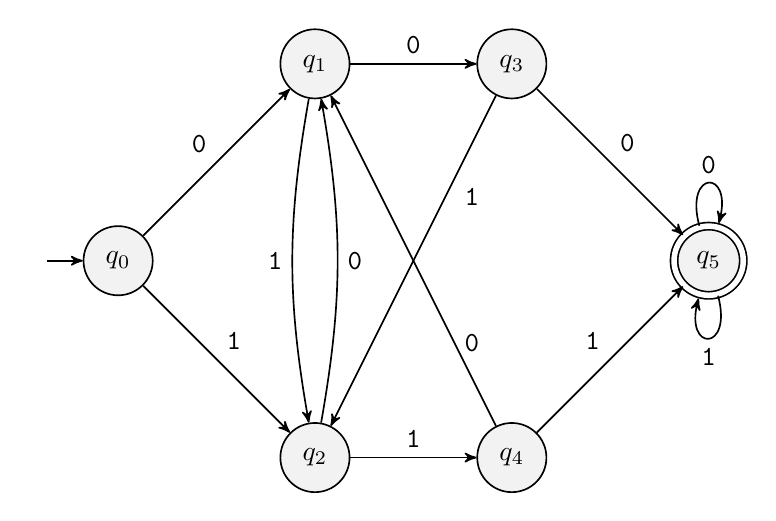
\begin{tikzpicture}
    \node[state, initial] (q0) {$q_0$};
    \node[state, right of=q0, above of=q0] (q1) {$q_1$};
    \node[state, right of=q1, below of=q0] (q2) {$q_2$};
    \node[state, right of=q1] (q3) {$q_3$};
    \node[state, right of=q2] (q4) {$q_4$};
    \node[state, right of=q3, below of=q3, accepting] (q5) {$q_5$};
    \draw (q0) edge node {\tt 0} (q1);
    \draw (q0) edge node {\tt 1} (q2);
    \draw (q1) edge node {\tt 0} (q3);
    \draw (q1) edge[left, bend right=10] node {\tt 1} (q2);
    \draw (q2) edge[right, bend right=10] node {\tt 0} (q1);
    \draw (q2) edge node {\tt 1} (q4);
    \draw (q3) edge node {\tt 0} (q5);
    \draw (q3) edge[near start] node {\tt 1} (q2);
    \draw (q4) edge[right, near start] node {\tt 0} (q1);
    \draw (q4) edge node {\tt 1} (q5);
    \draw (q5) edge[loop above] node {\tt 0} (q5);
    \draw (q5) edge[loop below] node {\tt 1} (q5);
    
    \end{tikzpicture}
\end{center}

\end{document}
